\documentclass[11pt]{article}
\usepackage[T1]{fontenc}
\usepackage[utf8]{inputenc}
\usepackage{mathptmx}
\usepackage[margin=1in]{geometry}
\usepackage{amsmath,amssymb}
\usepackage{booktabs}
\usepackage{tabularx}
\usepackage{xcolor}
\usepackage{tikz}
\usetikzlibrary{arrows.meta,positioning}
\usepackage{listings}
\usepackage{enumitem}
\usepackage[hidelinks]{hyperref}

\definecolor{accent}{HTML}{2F6FB3}
\definecolor{good}{HTML}{2E8B57}
\definecolor{bad}{HTML}{C0392B}
\definecolor{undec}{HTML}{7F8C8D}

\lstset{basicstyle=\ttfamily\footnotesize, columns=fullflexible,
        keepspaces=true, frame=single, rulecolor=\color{black!25},
        xleftmargin=1em, xrightmargin=1em, breaklines=true, showstringspaces=false}

\newcommand{\Prem}{\mathrm{Prem}}
\newcommand{\Conc}{\mathrm{Conc}}
\newcommand{\Sub}{\mathrm{Sub}}
\newcommand{\Last}{\mathrm{LastDef}}
\newcommand{\cmd}[1]{\texttt{#1}}

\title{Replaying the News:\\
Defeasible Argumentation over Dated Evidence\\
for Countering Disinformation}
\author{Andrew Dougherty\\
\small FRDCSA Project\\
\small\texttt{552578+aindilis@users.noreply.github.com}}
\date{Proposal and system description, version 0.3 \quad 14 October 2026}

\begin{document}
\maketitle

\begin{center}
\fbox{\parbox{0.9\linewidth}{\small\textbf{Review status.} This paper, the
software and the case encodings were drafted by Claude (Anthropic) at the
author's direction on 14 October 2026. Case facts were checked against the
cited sources and every reported status against the running engine and its
regression tests. The author has looked over this draft but has not yet
verified its content.}}
\end{center}

\begin{abstract}
Readers form beliefs about a news story from the first accounts they see,
and rarely revisit those beliefs when later evidence overturns the
accounts. We describe the News Analysis System, which keeps a live
argument map of a story: every statement of record is stored with its
source and the moment it became public; defeasible rules combine
statements into arguments; and the arguments are evaluated under ASPIC+
with grounded semantics. Because evidence is dated, the state of any
story can be replayed as of any past moment, separating honest early
error from later failure to update. Every verdict is explained by the
arguments behind it, and for every verdict the system lists the evidence
whose defeat would change it. A working prototype, the Colloquy engine in
SWI-Prolog with three sourced demonstration cases, is distributed as
Debian packages. We give the formal model, the implementation, the case
studies, an evaluation plan, and \emph{conspiracy numbers}: for each
conclusion, the smallest number of sources that would have to be wrong
for it to change, together with a report of which verdicts depend on a
single priority judgement.
\end{abstract}

%======================================================================
\section{Introduction}

Disinformation succeeds less by persuading people of falsehoods than by
arriving first. An early account, often from the party with the most
immediate access and the most interest in the framing, sets what a
reader believes; contradicting evidence arrives later, scattered across
outlets, and seldom triggers a review of the original claims. Articles
are updated without notice. Repetition of one source by many outlets
looks like corroboration. Binary fact-check labels hide what a verdict
depends on, so a settled claim and one resting on a single unverified
statement look the same.

What a careful reader needs is not a verdict machine but a
bookkeeping machine: one that records what each conclusion depends on and
recomputes when the dependencies change. Formal argumentation provides
exactly this. A conclusion is accepted when some argument for it
survives every attack; when new evidence arrives, the arguments are
rebuilt and re-evaluated, and the reasons for any change are explicit.

This paper makes four contributions:
\begin{enumerate}[nosep]
\item A model of news evidence as dated, sourced premises in an ASPIC+
argumentation theory, with replay to any moment
(Section~\ref{sec:model}).
\item A working, packaged implementation with an explanation command
and a \emph{what-would-change-this} command (Section~\ref{sec:impl}).
\item Three case studies chosen to end three different ways: refuted, self-corrected,
and not established (Section~\ref{sec:cases}).
\item An epistemic stance of symmetric scrutiny, and an implemented
measure, the conspiracy number, that puts claims of hidden coordination
and their denials on the same quantitative footing, with a priority
sensitivity report (Section~\ref{sec:stance}).
\end{enumerate}

The system revives a 2018 proposal by the author, built on the news-monitor
and argument-system components of the FRDCSA project.

%======================================================================
\section{Related work}
\label{sec:related}

\paragraph{Claim extraction and fact verification.}
Loki~\cite{loki} decomposes text into claims, scores check-worthiness,
retrieves evidence and verifies each claim, keeping a human in the loop.
It produces per-claim verdicts without a dependency structure between
claims, and without a notion of how a verdict changes over time.

\paragraph{Propaganda technique detection.}
SemEval-2020 Task~11~\cite{semeval2020} established span-level detection
of persuasion techniques in news; recent tools apply large language
models to the same labels. These identify rhetoric, not truth: a
passage can use loaded language and be accurate.

\paragraph{Argument mining.}
MARGOT~\cite{margot} extracts claims and evidence from text, and the
ARG-tech group deployed argument mining to the public with the BBC's
Evidence Toolkit. Argument mining recovers the structure inside one
text; it does not reason across sources over time.

\paragraph{Crowd context.}
X's Community Notes ranks notes by agreement among raters who usually
disagree~\cite{birdwatch}, and publishes its code and data. Notes are
prose: they are not machine-checkable and do not compose.

\paragraph{Structured argumentation.}
Dung's abstract frameworks~\cite{dung} define acceptability over an
attack graph; ASPIC+~\cite{aspic} gives arguments internal structure
(premises, strict and defeasible rules) and distinguishes undermining,
rebutting and undercutting. Argumentation schemes and their critical
questions~\cite{walton} supply the patterns of presumptive reasoning
used in our rules. The Argument Interchange Format~\cite{aif} lets
argument graphs move between tools. Story-based approaches to legal
evidence~\cite{bex} combine arguments with competing narratives, which
is close to our proposed extension in Section~\ref{sec:future}.

\paragraph{Analytic environments.}
DARPA's AIDA program~\cite{aida} built semantic engines that generate
explicit alternative interpretations of events from multimedia sources
and keep competing hypotheses alive rather than committing early. Our
grounded semantics is the single most sceptical interpretation; the
preferred semantics planned for phase~1 enumerates the alternatives in
the same spirit.

\paragraph{The gap.}
None of these keeps a persistent store in which each claim is tied to a
dated source, claims are combined into structured arguments, and
acceptance is recomputed, with reasons, whenever evidence is added. That
join is what this system provides; extraction, technique detection and
crowd input can feed it rather than be rebuilt.

%======================================================================
\section{Formal model}
\label{sec:model}

We follow ASPIC+~\cite{aspic} in a simplified form.

\paragraph{Language and theory.}
Let $\mathcal{L}$ be a set of ground literals closed under a negation
$\neg$, with a symmetric contrariness relation $\bar{\ }$ such that
$\varphi$ and $\neg\varphi$ are contraries, and further pairs may be
declared. Literals of the form $\mathit{undercut}(r)$ name rules. An
argumentation theory is
\[
  T = (\mathcal{L},\ R_s,\ R_d,\ K_n,\ K_p,\ \pi,\ \delta)
\]
where $R_s$ and $R_d$ are strict and defeasible rules of the form
$\varphi_1,\dots,\varphi_n \Rightarrow \psi$; $K_n$ are axioms and $K_p$
ordinary premises; $\pi : R_d \cup K_p \to \mathbb{N}$ assigns
priorities; and $\delta : K_n \cup K_p \rightharpoonup \mathcal{T}$
assigns each statement of record the time it became public, where
$\mathcal{T}$ is a totally ordered set of timestamps.

\paragraph{Replay.}
For a moment $t$, the restricted theory $T_t$ keeps only the
statements public by $t$:
\[
  K_p^t = \{\varphi \in K_p \mid \delta(\varphi) \text{ undefined or } \delta(\varphi) \le t\},
\]
and likewise for $K_n$. All further definitions are relative to $T_t$.

\paragraph{Arguments.}
Every $\varphi \in K_n^t \cup K_p^t$ is an argument $A$ with
$\Conc(A)=\varphi$, $\Prem(A)=\{\varphi\}$, $\Sub(A)=\{A\}$. If
$A_1,\dots,A_n$ are arguments and $r : \Conc(A_1),\dots,\Conc(A_n)
\Rightarrow \psi$ is a rule, then $B = A_1,\dots,A_n \Rightarrow_r \psi$
is an argument with $\Conc(B)=\psi$, $\Prem(B)=\bigcup \Prem(A_i)$ and
$\Sub(B)=\bigcup\Sub(A_i)\cup\{B\}$, provided $\psi$ is not the
conclusion of any argument in $\bigcup\Sub(A_i)$. The last defeasible
rules of an argument are $\Last(B)=\{r\}$ if $r\in R_d$, and
$\bigcup\Last(A_i)$ if $r \in R_s$.

\paragraph{Attacks.}
$A$ attacks $B$ on $B' \in \Sub(B)$ if
\begin{itemize}[nosep]
\item (undermine) $B' = \varphi \in K_p^t$ and $\Conc(A)$ is a contrary of $\varphi$;
\item (rebut) $B'$ ends in $r\in R_d$ and $\Conc(A)$ is a contrary of $\Conc(B')$;
\item (undercut) $B'$ ends in $r\in R_d$ and $\Conc(A)=\mathit{undercut}(r)$.
\end{itemize}

\paragraph{Preferences.}
For sets of priorities $S_1,S_2$, the elitist ordering is
$S_1 \lhd S_2$ iff $S_1 \neq \emptyset$ and either $S_2=\emptyset$ or
$\min S_1 < \min S_2$. Under the last-link principle, $A \prec B$ iff
$\pi(\Last(A)) \lhd \pi(\Last(B))$, or both are empty and
$\pi(\Prem(A)\cap K_p) \lhd \pi(\Prem(B)\cap K_p)$.

\paragraph{Defeat.}
$A$ defeats $B$ if $A$ attacks $B$ on $B'$ by undercutting, or by
rebutting or undermining with $A \not\prec B'$.

\paragraph{Grounded labelling.}
Let $\mathcal{A}_t$ be the arguments of $T_t$ and $D$ the defeat
relation. Starting from $\mathit{In}=\mathit{Out}=\emptyset$, repeat
until no change:
\[
\begin{aligned}
\mathit{In}  &\leftarrow \mathit{In}  \cup \{A \mid \forall X\,(X D A \rightarrow X\in\mathit{Out})\},\\
\mathit{Out} &\leftarrow \mathit{Out} \cup \{A \mid \exists X\in\mathit{In}\,(X D A)\}.
\end{aligned}
\]
Arguments in neither set are undecided. This computes the grounded
extension~\cite{dung}, the least fixed point of the characteristic
function and the most sceptical of the standard semantics.

\paragraph{Statuses.}
For a literal $\varphi$ at moment $t$:
\[
\mathrm{Stat}_t(\varphi) =
\begin{cases}
\textsc{accepted}  & \exists A\in\mathit{In},\ \Conc(A)=\varphi\\
\textsc{refuted}   & \text{else } \exists A\in\mathit{In},\ \Conc(A)\text{ a contrary of }\varphi\\
\textsc{none}      & \text{else no argument concludes }\varphi\\
\textsc{contested} & \text{else some argument for }\varphi\text{ is undecided}\\
\textsc{defeated}  & \text{otherwise.}
\end{cases}
\]
The distinction between \textsc{refuted} and \textsc{defeated} carries
the system's main epistemic point: a claim whose every argument has been
undercut is \emph{not established}, which is different from shown false.
Figure~\ref{fig:bridge} shows the labelling for a small fictional example.

%======================================================================
\section{Implementation}
\label{sec:impl}

The engine, Colloquy, is one SWI-Prolog module of about 670 lines. A
\emph{case} is a Prolog file declaring premises, axioms, rules, critical
questions, contraries and the topics the case tracks. Each case is loaded
into its own module; the current case is a global variable; and the
labelling for each case and moment is memoised with tabling. The engine
uses no \cmd{assert} or \cmd{retract}.

Argument construction is a forward closure: starting from the available
premises, every rule whose antecedents are concluded by existing
arguments is applied, skipping circular applications, until no new
argument appears. Defeat is computed over all pairs and sub-arguments,
then the grounded labelling is iterated to its fixed point. Exhaustive
construction is adequate for cases of a few dozen premises and rules.

A short excerpt from a case file:
\begin{lstlisting}[language=Prolog]
p(city, city_says_bridge_open, '2026-03-01T08:30', city, 3,
  'City traffic department: bridge open, a minor accident was cleared', []).

defeasible(r_city, [city_says_bridge_open], neg(bridge_collapsed),
           [prio(3), label('the authority responsible reports it open')]).
critical_question(r_photo_current, 'Has the photo appeared anywhere before?').
\end{lstlisting}

The command-line front end offers:
\begin{description}[nosep,font=\ttfamily\normalsize]
\item[status] the status of every topic at a moment;
\item[explain] every argument for a literal, its label, its premises with
  sources, and its defeaters;
\item[whatif] for an accepted literal, the premises, defeasible rules and
  critical questions whose defeat would change it;
\item[timeline] a replay listing, for each moment at which evidence
  arrived, the new evidence and every status that changed;
\item[robustness] conspiracy numbers and priority sensitivity
  (Section~\ref{sec:stance});
\item[aif] export of the argument graph in AIF JSON~\cite{aif}.
\end{description}

The system is packaged as three Debian packages: \cmd{colloquy} (the
engine), \cmd{news-analysis-cases} (sourced cases and regression tests)
and \cmd{news-analysis-system} (a metapackage and demonstration script).
Twenty-five regression tests check expected statuses at given moments,
conspiracy numbers and priority flips, and run at build time.

\begin{figure}[t]
\centering
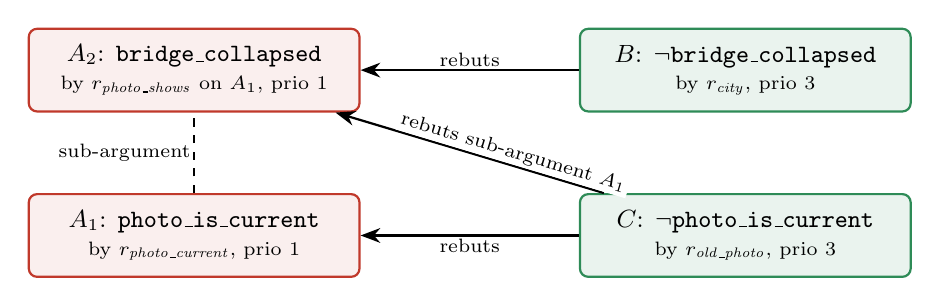
\begin{tikzpicture}[
  arg/.style={draw, rounded corners=3pt, align=center, font=\small,
              minimum width=4.2cm, minimum height=1.05cm, line width=0.8pt},
  argin/.style={arg, draw=good, fill=good!10},
  argout/.style={arg, draw=bad, fill=bad!8},
  def/.style={-{Stealth[length=2.5mm]}, line width=0.8pt},
  lab/.style={font=\scriptsize, fill=white, inner sep=1pt}]
\node[argout] (A1) at (0,0) {$A_1$: \texttt{photo\_is\_current}\\[-1pt]\scriptsize by $r_{\mathit{photo\_current}}$, prio 1};
\node[argout] (A2) at (0,2.1) {$A_2$: \texttt{bridge\_collapsed}\\[-1pt]\scriptsize by $r_{\mathit{photo\_shows}}$ on $A_1$, prio 1};
\node[argin] (B)  at (7,2.1) {$B$: $\neg$\texttt{bridge\_collapsed}\\[-1pt]\scriptsize by $r_{\mathit{city}}$, prio 3};
\node[argin] (C)  at (7,0) {$C$: $\neg$\texttt{photo\_is\_current}\\[-1pt]\scriptsize by $r_{\mathit{old\_photo}}$, prio 3};
\draw[def] (B) -- node[lab, above] {rebuts} (A2);
\draw[def] (C) -- node[lab, below] {rebuts} (A1);
\draw[def] (C) -- node[lab, sloped, above, pos=0.35] {rebuts sub-argument $A_1$} (A2);
\draw[dashed, line width=0.6pt] (A1) -- node[lab, left] {sub-argument} (A2);
\end{tikzpicture}
\caption{The fictional bridge rumour at 08:45. Green arguments are
\textsc{in}, red are \textsc{out}. $A_2$'s rebuttals of $B$ fail because
$A_2$'s last defeasible rule has lower priority, so $B$ and $C$ are
undefeated. Both topics are \textsc{refuted}.}
\label{fig:bridge}
\end{figure}

%======================================================================
\section{Case studies}
\label{sec:cases}

Three cases ship with the prototype. They were chosen to end three
different ways, so that readers see the engine refute, wait, and
withhold. Facts are taken from the cited reports; priorities follow a
published scale (1: inference from behaviour with other explanations or
unmeasured impressions; 2: testimony by an interested party; 3:
official records, forensic reports; 4: independent measurement or
replication; 5: recordings, experimenters reporting their own error;
6: court verdicts).

\subsection{A fake image, refuted within the day}

On 22 May 2023 an apparently AI-generated image of smoke ``at the
Pentagon'' spread on Twitter at 10:06 Eastern, shared by paid-verified
accounts including one impersonating Bloomberg News; US stocks fell
sharply within minutes and rebounded~\cite{petapixel,npr}. The Arlington
County fire department and the Pentagon Force Protection Agency stated
there was no incident, and a Bellingcat analyst noted artifacts and the
absence of other witnesses~\cite{npr}.

\begin{center}\small
\begin{tabularx}{\linewidth}{@{}l X l@{}}
\toprule
Moment & New evidence & Change\\
\midrule
10:06 & Viral image & explosion, authentic image: \textsc{accepted}\\
10:10 & Stocks fall sharply & market reaction: \textsc{accepted}\\
by 18:19 & Official denial; image analysis; impostor accounts & explosion, authentic image: \textsc{refuted}\\
\bottomrule
\end{tabularx}
\end{center}

The denial's exact time was not reported, so it is dated by the
publication of the report that carried it, marked as an upper bound. At
10:06, \cmd{whatif} lists the critical questions a reader should have
asked: are there other images or firsthand witnesses, is the poster who
it claims to be, does the image show signs of generation. The evidence
that refuted the claim answered exactly those. The market reaction stays
accepted throughout: it shows that people believed the claim, not that
it was true.

\subsection{A scientific anomaly, self-corrected}

On 23 September 2011 the OPERA collaboration reported muon neutrinos
arriving about 60.7\,ns earlier than light would, at about six sigma, and
offered no theoretical interpretation~\cite{operawiki}. A November re-test
with short beam pulses on the same detector gave the same result. In
February 2012 the collaboration identified a loose fibre-optic link in
its GPS timing chain and a fast-running clock; in March the ICARUS
detector, on the same beam, measured a speed consistent with light; the
experiment's spokesperson and physics coordinator stepped down; and in
June corrected measurements were presented at Neutrino 2012 in
Kyoto~\cite{operawiki}.

\begin{center}\small
\begin{tabularx}{\linewidth}{@{}l X l@{}}
\toprule
Date & New evidence & Change\\
\midrule
2011-09-23 & OPERA measurement & faster than light: \textsc{contested}\\
2011-11-18 & Re-test, same apparatus & none\\
2012-02-23 & Fault found by the experimenters & \textsc{refuted}; fault: \textsc{accepted}\\
2012-03-16 & ICARUS replication & none\\
2012-03-30 & Leaders step down & none\\
2012-06-08 & Corrected results & none\\
\bottomrule
\end{tabularx}
\end{center}

The measurement and the background theory have equal priority, so each
defeats the other and the claim is undecided rather than dismissed. The
re-test adds an argument but no independent weight, since it shares the
original's timing chain; the engine's ``no change'' is the right reading.
The fault report undercuts both measurements, the theory's argument
becomes undefeated, and the claim is refuted. Later events change
nothing: the replication is redundant, and the resignations are not
evidence.

\subsection{A live claim, not established}

In October 2026 Ukrainian drones struck Yandex data centres; Yandex
reported its Sasovo and Vladimir sites out of operation, and President
Zelensky, asked about the strike, said Ukraine responds in
kind~\cite{liga1,euronews}. A Cloudflare Radar analysis found automated
traffic from Yandex's network down about 94\% on 11 October, a figure
that also counts legitimate crawlers and cannot show whether
Kremlin-linked bots were affected~\cite{euronews}. On 12 October
Zelensky said bot activity had fallen and social media had become less
hostile, citing no data~\cite{liga2}; users in several countries reported
fewer apparently automated political replies, with no verified
figures~\cite{euronews}; and the Lithuanian prime minister urged allies to
seek more such strikes~\cite{malaymail}.

\begin{center}\small
\begin{tabularx}{\linewidth}{@{}l X l@{}}
\toprule
Topic & Basis & Status (14 Oct)\\
\midrule
Strikes on data centres & Target and attacker both describe them & \textsc{accepted}\\
Automated traffic fell & Independent network measurement & \textsc{accepted}\\
Political bot activity fell & Testimony without data; unmeasured reports; traffic incl.\ crawlers & \textsc{defeated}\\
Fall caused by strikes & Depends on the previous row & \textsc{defeated}\\
Pro-Trump bots specifically & No source checked makes this claim & none\\
\bottomrule
\end{tabularx}
\end{center}

Each argument that bot activity fell is undercut for a different reason,
so the claim is not established, and nothing shows it false. The last
row records a version of the story that circulated in conversation but
appears in no source examined: the story people repeat is not always the
story the sources tell. Adding a hypothetical independent measurement of
political bot posts, at priority~4, changes both middle rows to
\textsc{accepted}; more testimony would not.

%======================================================================
\section{Epistemic stance and conspiracy numbers}
\label{sec:stance}

\paragraph{Symmetric scrutiny.}
Hypotheses about coordination, motive or concealment are encoded like
any other claim, and so are their denials. ``This story was timed to
distract from another'' and ``the timing is coincidental'' are both
claims that need premises; neither is the default. Symmetric scrutiny
is not equal credence: base rates are evidence too, entered as sourced
premises open to attack.

\paragraph{Symmetric procedure, asymmetric outcomes.}
Two features of the method tend to favour less-coordinated explanations,
without any built-in stance. First, a hypothesis that reads missing
evidence as proof of concealment can absorb any observation; every
hidden-coordination hypothesis therefore carries the critical question
\emph{what observation would count against this?}, and one with no
answer makes no risky prediction. Second, documented conspiracies
surface through ordinary evidence---documents, whistleblowers, court
records---which the engine already weighs.

\paragraph{Conspiracy numbers.}
McAllester's conspiracy numbers~\cite{mcallester} measure, for a
game-tree search, how many leaf values would have to change to change
the value at the root. We propose the analogue for news. For a literal
$\varphi$ with status $s=\mathrm{Stat}_t(\varphi)$ in theory $T_t$,
\[
  \mathrm{cn}_t(\varphi) \;=\; \min\bigl\{\, |\sigma(S)| \;:\; S \subseteq K_p^t,\;
  \mathrm{Stat}_t^{\,T_t \setminus S}(\varphi) \neq s \,\bigr\},
\]
where $T_t\setminus S$ removes the premises $S$, and $\sigma(S)$ is the
set of \emph{independent sources} behind them, so that one outlet
repeating another counts once. The conspiracy number is the smallest
number of independent sources that would have to be wrong, mistaken or
colluding for the verdict to change.

The measure treats both directions alike. A claim that one interested
party is lying has a conspiracy number of one, and suspecting it is
reasonable. A claim that requires forty independent sources to be
coordinated has a conspiracy number of forty, and the engine can say so
without calling it absurd. The same machinery answers the question an
investigator asks when some evidence is known to be bad: which smallest
set of premises, if set aside, yields a coherent account? Computing
$\mathrm{cn}$ is a minimal hitting-set problem and NP-hard in general;
for cases of the present size, enumeration in increasing size is
practical, and that is what the \cmd{robustness} command does. Each
premise is its own source unless premises are grouped by a declared
origin. For a literal that is not accepted, the command also reports the
smallest set whose removal would make it accepted, or that none would.

\paragraph{Priority sensitivity.}
Priorities are the least checkable part of a case. The same command
moves each rule and premise priority up and down by one, recomputes, and
lists every verdict that changes.

\paragraph{Results on the demo cases.}
\begin{center}\small
\begin{tabularx}{\linewidth}{@{}l l l X@{}}
\toprule
Literal (moment) & Status & cn & To become accepted\\
\midrule
Explosion at Pentagon (18:19) & \textsc{refuted} & 1 & 3 sources: officials, image analysis, impostor record\\
Faster than light (June 2012) & \textsc{refuted} & 3 & 4 sources, including relativity itself\\
Political bot activity fell & \textsc{defeated} & 1 & 1 source: the crawler caveat\\
Pro-Trump bots specifically & none & --- & no removal suffices; needs new evidence\\
\bottomrule
\end{tabularx}
\end{center}
The table separates claims a single doubt would revive (the bot-activity
claim is one checkable fact from established) from claims that would
need several independent sources to fail together, and from claims no
amount of doubt can establish. On the latest evidence no verdict in any
case changes when a single priority moves by one; in September 2011 the
OPERA verdict changes under all four one-step moves of the measurement
and theory priorities, which makes explicit that the contested verdict
rested on judging them equally reliable.

%======================================================================
\section{Evaluation plan}
\label{sec:eval}

The test is retrospective replay on cases whose outcome is now known,
with a corpus balanced so that the system is not rewarded for doubting
every first account.
\begin{enumerate}[nosep]
\item \emph{Early-warning value.} Among conclusions accepted at first
report, compare how often those later refuted had an unanswered critical
question with how often those that held up did.
\item \emph{What-would-change hit rate.} For each actual reversal, check
whether the defeating evidence fell under an attack point that
\cmd{whatif} listed before it appeared.
\item \emph{No false reversals.} In cases where the first account held,
count conclusions the engine marked refuted; the target is zero.
\item \emph{Extraction agreement.} Compare premises and rules proposed by
a language-model extractor with hand encodings by two independent
annotators.
\item \emph{Reader study.} Give readers the argument view or the article
alone, and ask what evidence would change their view of the story;
score the specificity and correctness of the answers.
\end{enumerate}

%======================================================================
\section{Risks}

\begin{center}\small
\begin{tabularx}{\linewidth}{@{}>{\raggedright\arraybackslash}p{0.33\linewidth} X@{}}
\toprule
Risk & Mitigation\\
\midrule
Whoever sets the priorities sets the verdict & A published, per-case priority scale; a sensitivity report showing which verdicts flip when one priority moves by one\\
A corpus of reversals teaches distrust of all official accounts & Half of all cases are ones where the first account held; ``no false reversals'' is a hard target\\
The extractor invents or misreads claims & Extracted items enter as premises tagged with their model, attackable like any other; nothing is published without review\\
The tool amplifies motive or conspiracy claims & Symmetric scrutiny, the falsifiability critical question, conspiracy numbers, and named proof standards\\
Coordinated accounts flood shared questions & A peer question counts only if it cites a source; trust is each reader's own\\
Cases name real people & Only public-record facts, each with source and date\\
\bottomrule
\end{tabularx}
\end{center}

%======================================================================
\section{Roadmap}
\label{sec:future}

\begin{description}[nosep]
\item[Phase 1 (months 1--3)] Preferred semantics, so that every coherent
interpretation the evidence allows is listed, as in AIDA~\cite{aida};
rationality checks~\cite{caminada}; proof standards as a parameter;
faster conspiracy numbers for larger cases; twenty cases, half where the
first account held.
\item[Phase 2 (3--6)] A language-model extractor that proposes premises,
rules and attacks as a case file for human review. The language model
proposes; only the logic engine decides acceptance.
\item[Phase 3 (6--9)] An archive bridge: each premise points at a dated,
hashed web capture, and replay reads captures rather than live pages.
\item[Phase 4 (9--12)] A reader view showing status, explanation and
what would change it; signed peer questions; AIF round-trip with
existing argumentation tools.
\end{description}

%======================================================================
\section{Conclusion}

A news story is a sequence of claims with sources and times. Treating it
as a defeasible argumentation theory with dated premises gives readers
three things a verdict cannot: the reasons behind each conclusion, the
history of how those reasons changed, and the specific evidence that
would change them next. The prototype shows that this works on real
cases, with a small engine and a plain file format, and that it can say
the three different things a careful analyst says: this is false, this
was mistaken and has been corrected, and this has not been established.

\paragraph{Acknowledgements.}
The prototype, its case encodings and this paper were drafted by
Claude (Anthropic), working from the author's 2018 proposal and
direction; see the review status note on the first page.

%======================================================================
\begin{thebibliography}{99}\small

\bibitem{dung}
P.~M. Dung.
On the acceptability of arguments and its fundamental role in
nonmonotonic reasoning, logic programming and n-person games.
\emph{Artificial Intelligence}, 77(2):321--357, 1995.

\bibitem{aspic}
S.~Modgil and H.~Prakken.
The ASPIC+ framework for structured argumentation: a tutorial.
\emph{Argument \& Computation}, 5(1):31--62, 2014.

\bibitem{caminada}
M.~Caminada and L.~Amgoud.
On the evaluation of argumentation formalisms.
\emph{Artificial Intelligence}, 171(5--6):286--310, 2007.

\bibitem{walton}
D.~Walton, C.~Reed and F.~Macagno.
\emph{Argumentation Schemes}.
Cambridge University Press, 2008.

\bibitem{aif}
C.~Ches\~nevar, J.~McGinnis, S.~Modgil, I.~Rahwan, C.~Reed, G.~Simari,
M.~South, G.~Vreeswijk and S.~Willmott.
Towards an argument interchange format.
\emph{The Knowledge Engineering Review}, 21(4):293--316, 2006.

\bibitem{bex}
F.~J. Bex.
\emph{Arguments, Stories and Criminal Evidence: A Formal Hybrid Theory}.
Springer, 2011.

\bibitem{mcallester}
D.~A. McAllester.
Conspiracy numbers for min-max search.
\emph{Artificial Intelligence}, 35(3):287--310, 1988.

\bibitem{aida}
DARPA.
Active Interpretation of Disparate Alternatives (AIDA).
\url{https://www.darpa.mil/research/programs/active-interpretation-of-disparate-alternatives}.

\bibitem{loki}
H.~Li, X.~Han, H.~Wang, Y.~Wang, M.~Wang, R.~Xing, Y.~Geng, Z.~Zhai,
P.~Nakov and T.~Baldwin.
Loki: an open-source tool for fact verification.
In \emph{Proc.\ COLING 2025: System Demonstrations}, 2025.

\bibitem{semeval2020}
G.~Da San Martino, A.~Barr\'on-Cede\~no, H.~Wachsmuth, R.~Petrov and
P.~Nakov.
SemEval-2020 Task 11: Detection of propaganda techniques in news
articles.
In \emph{Proc.\ SemEval}, 2020.

\bibitem{margot}
M.~Lippi and P.~Torroni.
MARGOT: a web server for argumentation mining.
\emph{Expert Systems with Applications}, 65:292--303, 2016.

\bibitem{birdwatch}
S.~Wojcik, S.~Hilgard, N.~Judd, D.~Mocanu, S.~Ragain, M.~B.~F. Hunzaker,
K.~Coleman and J.~Baxter.
Birdwatch: crowd wisdom and bridging algorithms can inform understanding
and reduce the spread of misinformation.
arXiv:2210.15723, 2022.

\bibitem{npr}
NPR.
Fake viral images of an explosion at the Pentagon were probably created
by AI. 22 May 2023.
\url{https://www.npr.org/2023/05/22/1177590231/fake-viral-images-of-an-explosion-at-the-pentagon-were-probably-created-by-ai}.

\bibitem{petapixel}
PetaPixel.
AI-generated image of Pentagon explosion caused markets to dip.
22 May 2023.
\url{https://petapixel.com/2023/05/22/ai-generated-image-of-pentagon-explosion-caused-markets-to-dip/}.

\bibitem{operawiki}
Wikipedia.
2011 OPERA faster-than-light neutrino anomaly.
\url{https://en.wikipedia.org/wiki/2011_OPERA_faster-than-light_neutrino_anomaly}.

\bibitem{euronews}
Euronews.
Did Ukrainian strikes on Yandex data centres cause Russian bot activity
to plummet? 12 October 2026.
\url{https://euronews.com/2026/10/12/did-ukrainian-strikes-on-yandex-data-centres-cause-russian-bot-activity-to-plummet}.

\bibitem{liga1}
LIGA.net.
``We always respond in kind.'' Zelenskyy confirmed the strike on a
Russian data center. 8 October 2026.
\url{https://news.liga.net/en/war/news/we-always-respond-in-kind-zelenskyy-confirmed-the-strike-on-a-russian-data-center}.

\bibitem{liga2}
LIGA.net.
Attacks on Yandex data centers have reduced bot activity on social
media: Zelenskyy. 12 October 2026.
\url{https://news.liga.net/en/amp/politics/news/attacks-on-yandex-data-centers-have-reduced-bot-activity-on-social-media-zelenskyy}.

\bibitem{malaymail}
Malay Mail.
Hit more Russian data centres, says Lithuanian PM. 12 October 2026.
\url{https://malaymail.com/news/world/2026/10/12/hit-more-russian-data-centres-says-lithuanian-pm/238860}.

\end{thebibliography}
\end{document}
